\subsection{Backpropagation}

\begin{frame}
\frametitle{Backpropagation}

\begin{itemize}

\item{Liegt Kostenfunktion zugrunde}

\note[item]{Kostenfunktion wie bei Gradientenabstieg / Adeline}
\note[item]{Unterschied: Hier mehrschichtiges Netz}
\note[item]{1970er entwickelt, 1986 von Rummelhart, Hilten und Williams in Paper bekannt gemacht}
\note[item]{Gradientenabstieg grob erläutert, ausgeblieben - Anwendung im mehrschichtigen Netz und mehrdimensionale Kostenfunktion}
\end{itemize}
\end{frame}



\begin{frame}
\frametitle{Notation}

\begin{figure}
	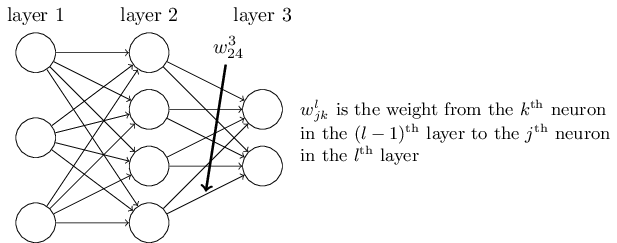
\includegraphics[width=\linewidth]{./aktuelleEntwicklung/backpropagation/img/weight_notation}
\end{figure}

\note[item]{l: Exponent, steht für die Schicht}
\note[item]{l - 1, weil man stets von hinten nach vorne schaut}
\note[item]{Eingabe wird auch als eigene Schicht verstanden}
\note[item]{j: Index Zielneuron}
\note[item]{k: Index Startneuron}

\end{frame}

\begin{frame}
\frametitle{Notation}

\begin{figure}
	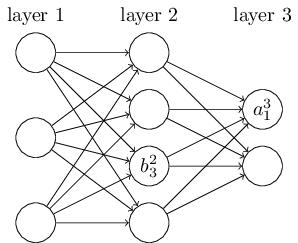
\includegraphics[width=.6\linewidth]{./aktuelleEntwicklung/backpropagation/img/biasAct_notation}
	
\note[item]{Ähnlich zu Gewichtsnotation}
\note[item]{l bezieht sich hierbei jedoch auf aktuelle Schicht}
\note[item]{j wie gehabt Index in Schicht}
\note[item]{Notation gilt auch für Aktivierung a}

\end{figure}

\begin{itemize}
\item Zusammensetzung der Aktivierung: 
\inlineeq{a^{l}_j = \sigma\left( \sum_k w^{l}_{jk} a^{l-1}_k + b^l_j \right)}

\end{itemize}

\end{frame}


\begin{frame}
\frametitle{Zusammensetzung der Aktivierung} 

\begin{itemize}
\item Zusammensetzung der Aktivierung: 
\inlineeq{a^{l}_j = \sigma\left( \sum_k w^{l}_{jk} a^{l-1}_k + b^l_j \right)}
\end{itemize}

\begin{itemize}
\item Vektorielle Darstellung der Aktivierung: 
\inlineeq{a^l = \sigma(z^l)}
\note[item]{Wichtig: $\sigma$ bezieht sich auf Vektor $\Rightarrow$ Vektorielle Funktion}
\note[item]{Jede Komponente einzeln mit $\sigma$ verarbeitet}
\end{itemize}

\begin{itemize}
\item Gewichtete Eingabe (\emph{Z}-Wert): \inlineeq{  z^l = w^l a^{l-1}+b^l}
\note[item]{Abstraktion vom Ausgabewert vor der Aktivierungsfkt. hilft später beim Ableiten}

\comment{
\item Vektorisierte Funktion (2-dim. Beispiel): 
\begin{align*}
f(x) \Rightarrow f\left(\left[ \begin{array}{c} x_1 \\ x_2 \end{array} \right] \right)
   = \left[ \begin{array}{c} f(x_1) \\ f(x_2) \end{array} \right]
\end{align*}}




\end{itemize}

\end{frame}

